\documentclass{article}\usepackage[]{graphicx}\usepackage[]{color}
%% maxwidth is the original width if it is less than linewidth
%% otherwise use linewidth (to make sure the graphics do not exceed the margin)
\makeatletter
\def\maxwidth{ %
  \ifdim\Gin@nat@width>\linewidth
    \linewidth
  \else
    \Gin@nat@width
  \fi
}
\makeatother

\definecolor{fgcolor}{rgb}{0.345, 0.345, 0.345}
\newcommand{\hlnum}[1]{\textcolor[rgb]{0.686,0.059,0.569}{#1}}%
\newcommand{\hlstr}[1]{\textcolor[rgb]{0.192,0.494,0.8}{#1}}%
\newcommand{\hlcom}[1]{\textcolor[rgb]{0.678,0.584,0.686}{\textit{#1}}}%
\newcommand{\hlopt}[1]{\textcolor[rgb]{0,0,0}{#1}}%
\newcommand{\hlstd}[1]{\textcolor[rgb]{0.345,0.345,0.345}{#1}}%
\newcommand{\hlkwa}[1]{\textcolor[rgb]{0.161,0.373,0.58}{\textbf{#1}}}%
\newcommand{\hlkwb}[1]{\textcolor[rgb]{0.69,0.353,0.396}{#1}}%
\newcommand{\hlkwc}[1]{\textcolor[rgb]{0.333,0.667,0.333}{#1}}%
\newcommand{\hlkwd}[1]{\textcolor[rgb]{0.737,0.353,0.396}{\textbf{#1}}}%
\let\hlipl\hlkwb

\usepackage{framed}
\makeatletter
\newenvironment{kframe}{%
 \def\at@end@of@kframe{}%
 \ifinner\ifhmode%
  \def\at@end@of@kframe{\end{minipage}}%
  \begin{minipage}{\columnwidth}%
 \fi\fi%
 \def\FrameCommand##1{\hskip\@totalleftmargin \hskip-\fboxsep
 \colorbox{shadecolor}{##1}\hskip-\fboxsep
     % There is no \\@totalrightmargin, so:
     \hskip-\linewidth \hskip-\@totalleftmargin \hskip\columnwidth}%
 \MakeFramed {\advance\hsize-\width
   \@totalleftmargin\z@ \linewidth\hsize
   \@setminipage}}%
 {\par\unskip\endMakeFramed%
 \at@end@of@kframe}
\makeatother

\definecolor{shadecolor}{rgb}{.97, .97, .97}
\definecolor{messagecolor}{rgb}{0, 0, 0}
\definecolor{warningcolor}{rgb}{1, 0, 1}
\definecolor{errorcolor}{rgb}{1, 0, 0}
\newenvironment{knitrout}{}{} % an empty environment to be redefined in TeX

\usepackage{alltt}
\usepackage{natbib}



\IfFileExists{upquote.sty}{\usepackage{upquote}}{}
\begin{document}
\title{Frankenstein's Wordcloud}
\author{Bill Fisher}
\maketitle

\begin{abstract}
In this article, we construct a wordcloud using the tidytext R package for Mary Wollstonecraft (Godwin) Shelley's Frankenstein, or the Modern Prometheus.
\end{abstract}

\textit{Frankenstein, or the Modern Prometheus} (or simply, Frankenstein for short), is a novel written by English author Mary Shelley (1797-1851) that tells the story of Victor Frankenstein, a young scientist who creates a grotesque but sapient creature in an unorthodox scientific experiment. Shelley started writing the story when she was 18, and the first edition of the novel was published in London in 1818, when she was 20.\footnote{The novel was originally published anonymously. Her name first appeared on the second edition, published in France in 1823.}  The book was later published around the world.\citep{Wikipedia}

\section{The GutenbergR package}
There is a package called GutenbergR whichholds the text of many novels to be deciphered using R.  One first has to install this package and bring it in with the library function.  Once loaded, we will find our book and download it.\footnote{You can search the database for the title of Frankenstein using the following codeline: gutenberg\_works(str\_detect(title,'Frankenstein'))} Once downloaded, we can store it in our dataframe.

\begin{knitrout}
\definecolor{shadecolor}{rgb}{0.969, 0.969, 0.969}\color{fgcolor}\begin{kframe}
\begin{alltt}
\hlkwd{library}\hlstd{(gutenbergr)}
\hlstd{frankenstein}\hlkwb{<-}\hlkwd{gutenberg_download}\hlstd{(}\hlnum{84}\hlstd{)}
\hlstd{frankenstein}
\end{alltt}
\begin{verbatim}
## # A tibble: 7,244 x 2
##    gutenberg_id                                 text
##           <int>                                <chr>
##  1           84                        Frankenstein,
##  2           84                                     
##  3           84             or the Modern Prometheus
##  4           84                                     
##  5           84                                     
##  6           84                                   by
##  7           84                                     
##  8           84 Mary Wollstonecraft (Godwin) Shelley
##  9           84                                     
## 10           84                                     
## # ... with 7,234 more rows
\end{verbatim}
\end{kframe}
\end{knitrout}

\noindent The dataframe, frankenstein, now contains our book but we still need to clean up the data.  Breaking it down into two major steps, we need to  clear the clutter at the beginning of the book and we need to erase the word  "chapter" from the beginning of each chapter.  To accomplish this, we run the following code:

\begin{knitrout}
\definecolor{shadecolor}{rgb}{0.969, 0.969, 0.969}\color{fgcolor}\begin{kframe}
\begin{alltt}
\hlkwd{library}\hlstd{(stringr)}
\hlkwd{library}\hlstd{(dplyr)}

\hlstd{frankenstein}\hlkwb{<-}\hlstd{frankenstein[}\hlnum{12}\hlopt{:}\hlnum{7244}\hlstd{,]}
\hlstd{frankenstein}
\end{alltt}
\begin{verbatim}
## # A tibble: 7,233 x 2
##    gutenberg_id
##           <int>
##  1           84
##  2           84
##  3           84
##  4           84
##  5           84
##  6           84
##  7           84
##  8           84
##  9           84
## 10           84
## # ... with 7,223 more rows, and 1 more variables: text <chr>
\end{verbatim}
\begin{alltt}
\hlstd{frankenstein}\hlkwb{<-}\hlstd{frankenstein}\hlopt
  \hlkwd{filter}\hlstd{(}\hlopt{!}\hlkwd{str_detect}\hlstd{(frankenstein}\hlopt{$}\hlstd{text,}\hlstr{'^CHAPTER'}\hlstd{))}
\hlstd{frankenstein}
\end{alltt}
\begin{verbatim}
## # A tibble: 7,233 x 2
##    gutenberg_id
##           <int>
##  1           84
##  2           84
##  3           84
##  4           84
##  5           84
##  6           84
##  7           84
##  8           84
##  9           84
## 10           84
## # ... with 7,223 more rows, and 1 more variables: text <chr>
\end{verbatim}
\end{kframe}
\end{knitrout}

\noindent Above, we change the start of our dataframe at the 12th line and include that and the last line.  We also use dplyr and the string detect function to elimintae all of the "chapters."

\noindent Next, we need to seperate our words.  We also need to discard the stop words.  To do this we run the following code:

\begin{knitrout}
\definecolor{shadecolor}{rgb}{0.969, 0.969, 0.969}\color{fgcolor}\begin{kframe}
\begin{alltt}
\hlkwd{library}\hlstd{(tidytext)}

\hlstd{words_df}\hlkwb{<-}\hlstd{frankenstein}\hlopt
  \hlkwd{unnest_tokens}\hlstd{(word,text)}
\hlstd{words_df}
\end{alltt}
\begin{verbatim}
## # A tibble: 75,165 x 2
##    gutenberg_id        word
##           <int>       <chr>
##  1           84      letter
##  2           84           1
##  3           84          st
##  4           84 petersburgh
##  5           84         dec
##  6           84        11th
##  7           84          17
##  8           84          to
##  9           84         mrs
## 10           84     saville
## # ... with 75,155 more rows
\end{verbatim}
\begin{alltt}
\hlstd{words_df}\hlkwb{<-}\hlstd{words_df}\hlopt
  \hlkwd{filter}\hlstd{(}\hlopt{!}\hlstd{(word} \hlopt \hlstd{stop_words}\hlopt{$}\hlstd{word))}
\hlstd{words_df}
\end{alltt}
\begin{verbatim}
## # A tibble: 27,274 x 2
##    gutenberg_id        word
##           <int>       <chr>
##  1           84      letter
##  2           84           1
##  3           84          st
##  4           84 petersburgh
##  5           84         dec
##  6           84        11th
##  7           84          17
##  8           84     saville
##  9           84     england
## 10           84     rejoice
## # ... with 27,264 more rows
\end{verbatim}
\end{kframe}
\end{knitrout}

\noindent Now that we have our words seperated, we need to get a count of each word so we can finish constructing our wordcloud.  To do this, we will once again use dplyr.

\begin{knitrout}
\definecolor{shadecolor}{rgb}{0.969, 0.969, 0.969}\color{fgcolor}\begin{kframe}
\begin{alltt}
\hlstd{word_freq}\hlkwb{<-}\hlstd{words_df}\hlopt
  \hlkwd{group_by}\hlstd{(word)}\hlopt
  \hlkwd{summarize}\hlstd{(}\hlkwc{count}\hlstd{=}\hlkwd{n}\hlstd{())}

\hlstd{word_freq}
\end{alltt}
\begin{verbatim}
## # A tibble: 6,561 x 2
##     word count
##    <chr> <int>
##  1   _i_     1
##  2     1     2
##  3    10     1
##  4    11     1
##  5  11th     2
##  6    12     1
##  7  12th     2
##  8    13     1
##  9  13th     1
## 10    14     1
## # ... with 6,551 more rows
\end{verbatim}
\end{kframe}
\end{knitrout}

\noindent Finally, we can construct our wordcloud.

\begin{knitrout}
\definecolor{shadecolor}{rgb}{0.969, 0.969, 0.969}\color{fgcolor}\begin{kframe}
\begin{alltt}
\hlkwd{library}\hlstd{(wordcloud)}
\hlkwd{wordcloud}\hlstd{(word_freq}\hlopt{$}\hlstd{word,word_freq}\hlopt{$}\hlstd{count,}\hlkwc{min.freq}\hlstd{=}\hlnum{27}\hlstd{)}
\end{alltt}
\end{kframe}
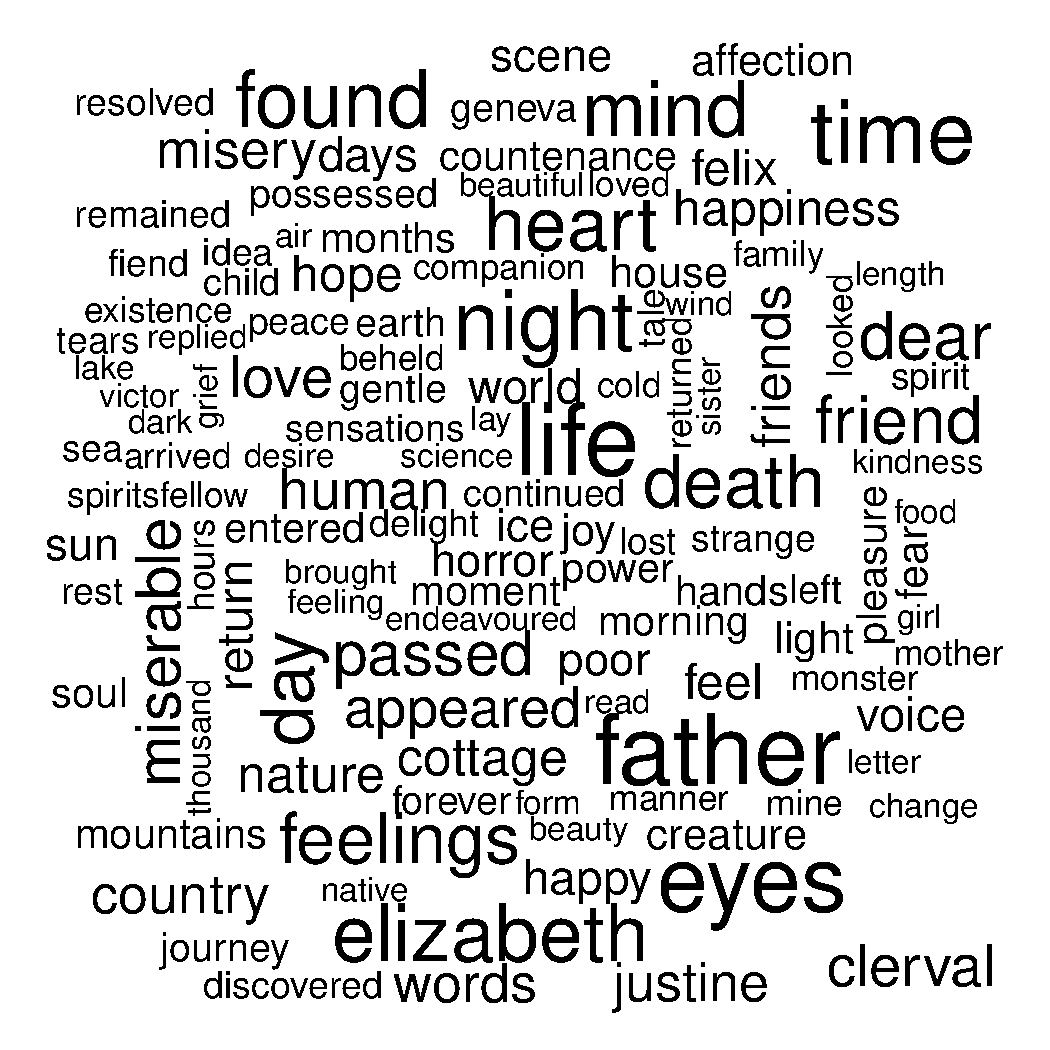
\includegraphics[width=\maxwidth]{figure/unnamed-chunk-6-1} 

\end{knitrout}

\noindent If we want, we can look at a certain sentiment's wordcloud.  For instance, using tidytext to define each word's sentiment, we can make a wordcloud out of each of Frankenstein's "fear" words with the following piece of code:

\begin{knitrout}
\definecolor{shadecolor}{rgb}{0.969, 0.969, 0.969}\color{fgcolor}\begin{kframe}
\begin{alltt}
\hlstd{nrc}\hlkwb{<-}\hlkwd{get_sentiments}\hlstd{(}\hlstr{'nrc'}\hlstd{)}

\hlstd{nrc_fear}\hlkwb{<-}\hlstd{nrc}\hlopt
  \hlkwd{filter}\hlstd{(sentiment}\hlopt{==}\hlstr{'fear'}\hlstd{)}

\hlstd{frankenstein_words_df}\hlkwb{<-}\hlkwd{inner_join}\hlstd{(nrc_fear,words_df)}

\hlstd{frank_fear_words}\hlkwb{<-}\hlstd{frankenstein_words_df}\hlopt
  \hlkwd{group_by}\hlstd{(word)}\hlopt
  \hlkwd{summarize}\hlstd{(}\hlkwc{count}\hlstd{=}\hlkwd{n}\hlstd{())}
\hlstd{frank_fear_words}
\end{alltt}
\begin{verbatim}
## # A tibble: 493 x 2
##         word count
##        <chr> <int>
##  1   abandon     2
##  2 abandoned     3
##  3     abhor     5
##  4 abhorrent     1
##  5  abortion     1
##  6   absence     8
##  7     abyss     1
##  8  accident     6
##  9  accursed     4
## 10   accused     7
## # ... with 483 more rows
\end{verbatim}
\begin{alltt}
\hlkwd{wordcloud}\hlstd{(frank_fear_words}\hlopt{$}\hlstd{word,frank_fear_words}\hlopt{$}\hlstd{count,}\hlkwc{min.freq}\hlstd{=}\hlnum{5}\hlstd{)}
\end{alltt}
\end{kframe}
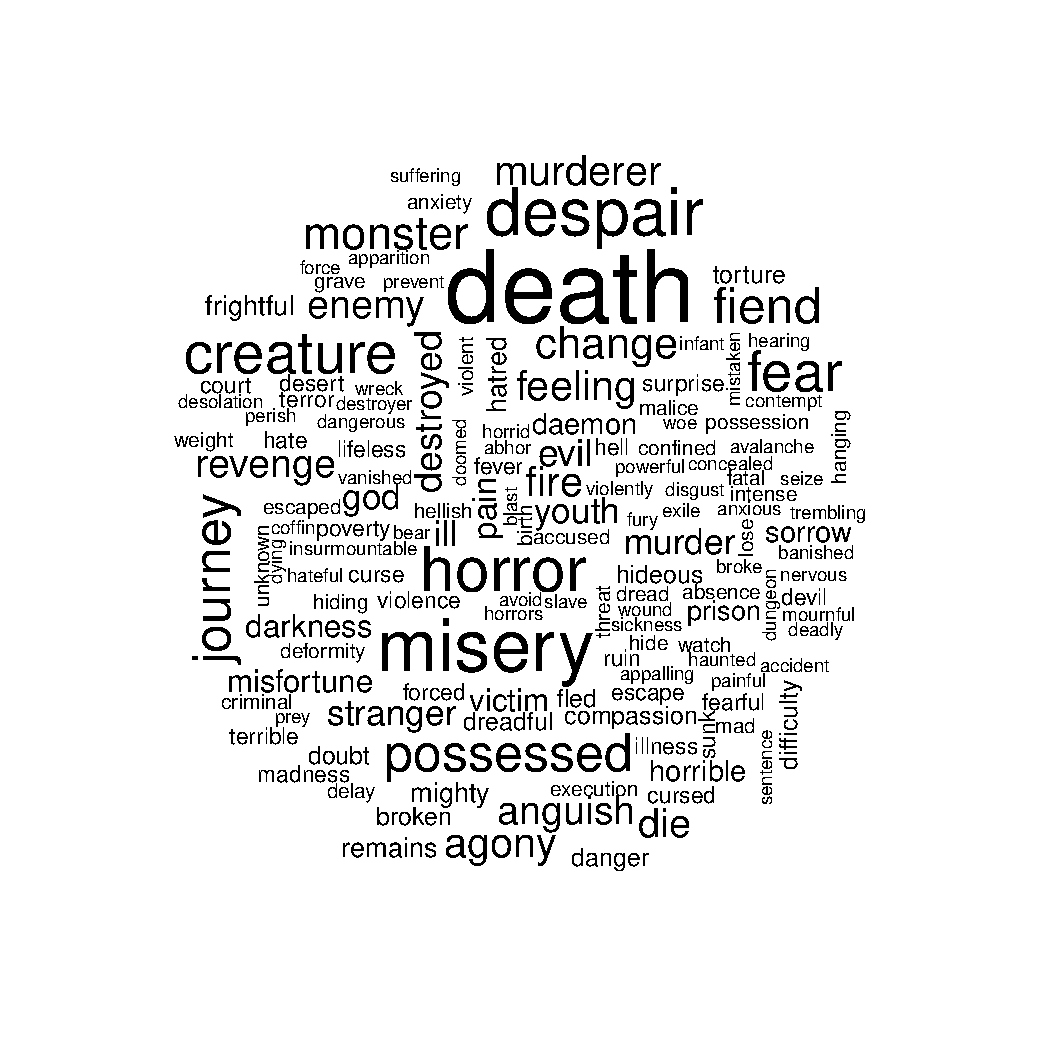
\includegraphics[width=\maxwidth]{figure/unnamed-chunk-7-1} 

\end{knitrout}


\bibliographystyle{apa}
\bibliography{frankenstein_wordcloud,packages}
\nocite{*}
\end{document}
